\section{Desarrollo de software}
Desarrollar software es una tarea complicada. No existe la bala de plata (\textit{El famoso paper, No silver bullet - Brooks}). La complejidad se compone por:

\begin{center}
$complejidad = complejidad\_solucion + complejidad\_problema$ 
\end{center}

Para atacarla, se utiliza abstracción para eliminar lo irrelevante y amplificar lo esencial, agrupar y ocultar (ignorar detalles y evitar verlos), restricciones para simplificar el enfoque, y la visibilidad (desacoplamiento).

La complejidad no esta en la solución, esta en el problema. Por lo que hay que desarrollar un buen criterio para resolver el problema. Se utilizan los mecanismos de descomposición (descubrir), abstracción (pensar en la esencia), y establecer jerarquías (inventar \textit{generalizaciones. Ej Documentos comerciales - son facturas, tickets y demás - El documento comercial por si solo no existe}). La descomposición y la abstracción se van a usar siempre en relación al negocio.

Es fundamental entender el problema para proponer un diseño que no se quede corto y que no sea algo complejo que sume al problema. 

\section{Modelo de dominio}
El modelo de dominio vive dentro del problema.  Este tiene patrones de análisis/colaboración y reglas del negocio, se arman \textit{tests}. Una vez que no se rompan estos \textit{tests}, se tiene el modelo de negocio.

\begin{figure}[!htb]
    \centering
    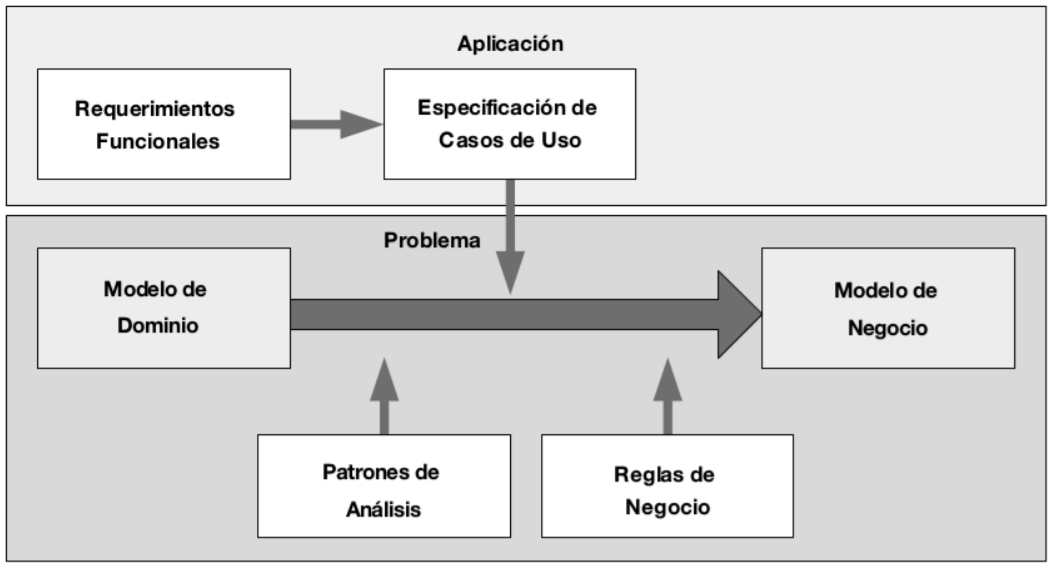
\includegraphics[width=0.8\textwidth]{img/ModeloDeDominio.PNG}
\end{figure}

En la aplicación están los requisitos funcionales \textit{Casos de uso, user stories}, prototipos de interfaces, diagramas de colaboración y secuencia. Estos van aportando al modelo de negocio.

\begin{figure}[!htb]
    \centering
    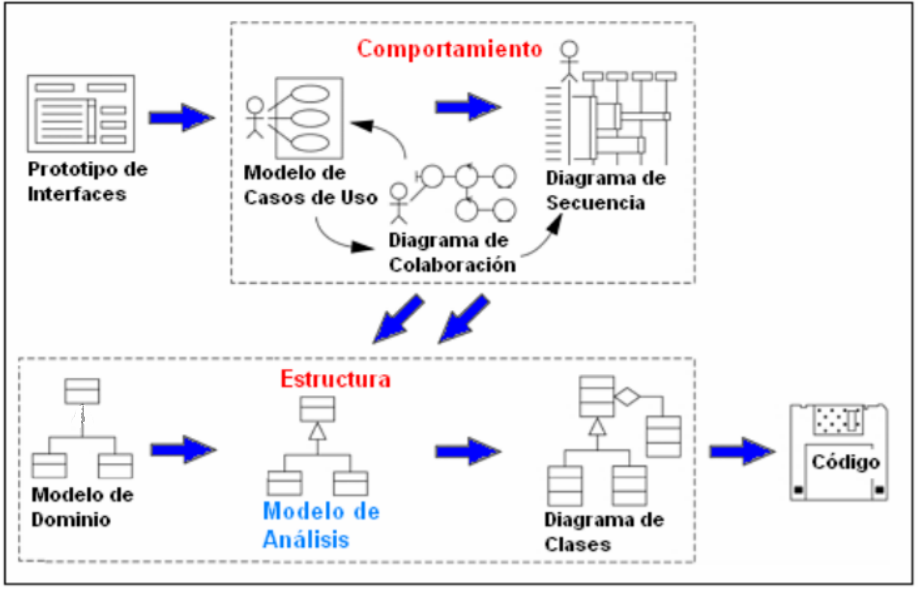
\includegraphics[width=0.8\textwidth]{img/ProcesoModeloDeDominio.PNG}
\end{figure}

Antes de tener el modelo de negocio, se inicia con un modelo de dominio, se busca descubrir. A esto le sigue un modelo de análisis que representa la dinámica del modelo de dominio. A partir de esto se llega al diagrama de clases.

\begin{itemize}
\item El modelo de negocio tiene como objetivo entender en detalle el negocio y sus reglas, para esto utiliza patrones de análisis o colaboración.
\item Se diferencia del Modelo de diseño, ya que este ultimo tiene como objetivo implementar una solución al problema planteado en el análisis mas las restricciones impuestas por los requisitos no funcionales. Utiliza los patrones de diseño.
\end{itemize}


\section{Patrones de análisis o colaboración}

\begin{figure}[!htb]
    \centering
    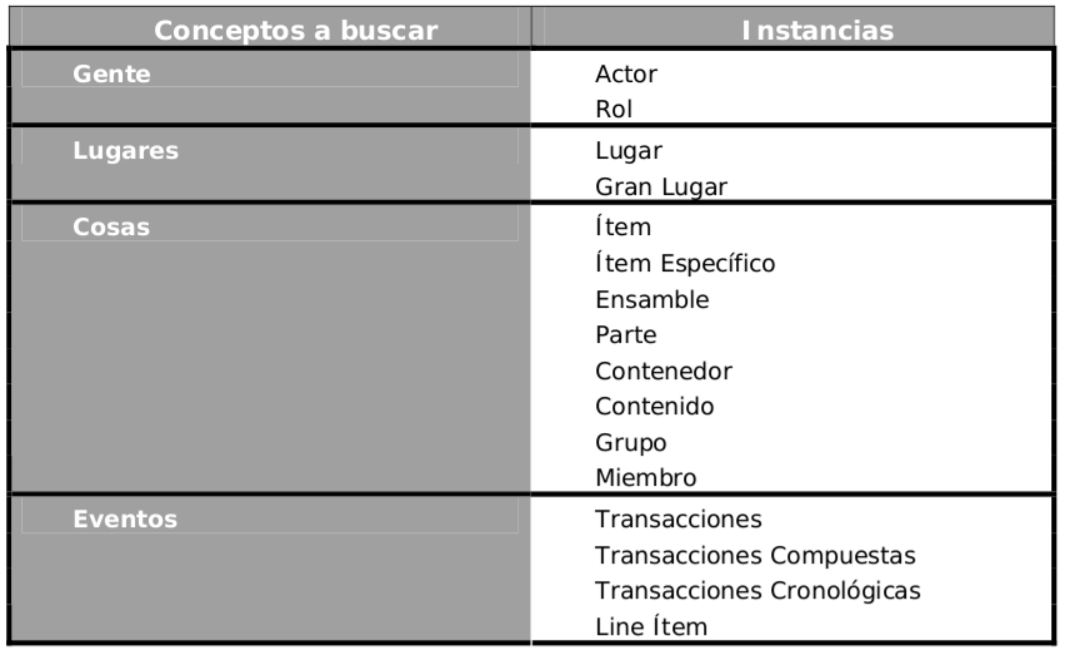
\includegraphics[width=0.8\textwidth]{img/PatronesAnalisisColaboracion.PNG}
    \caption{Las diferentes instancias que tenemos.}
\end{figure}

\begin{itemize}
\item Suelen aparecer de a dos relaciones. 
\item Tenemos 12 patrones en total, estos se usan para armar el modelo de dominio.
\item La idea es descubrir en base a ellos siguiendo los pasos que se van a mostrar después.
\item En esta etapa del modelo de dominio, no hay que usar interfaces y herencia, solo hay que usar los patrones de colaboración.
\item \textit{En las resoluciones de ejercicios, indicar que patrón se esta utilizando.} 
\end{itemize}

\newpage
\subsubsection*{Actor-Rol}
\begin{figure}[!htb]
    \centering
    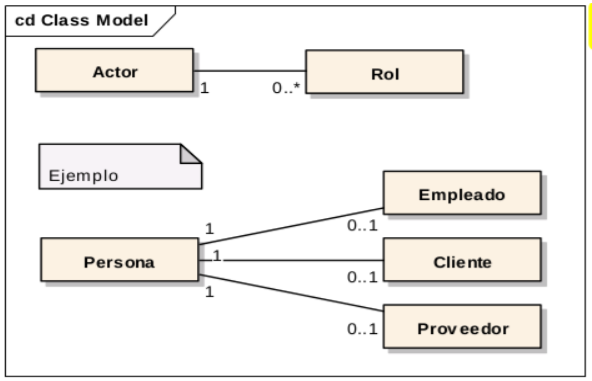
\includegraphics[width=0.6\textwidth]{img/PatronActorRol.PNG}
\end{figure}

\subsubsection*{GranLugar-Lugar}
\begin{figure}[!htb]
    \centering
    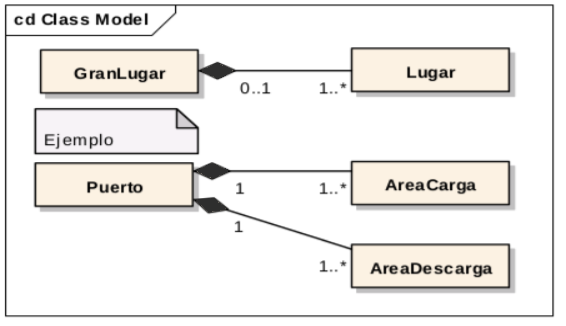
\includegraphics[width=0.6\textwidth]{img/PatronGranLugarLugar.PNG}
\end{figure}
\newpage
\subsubsection*{Item-ItemEspecifico}

\begin{figure}[!htb]
    \centering
    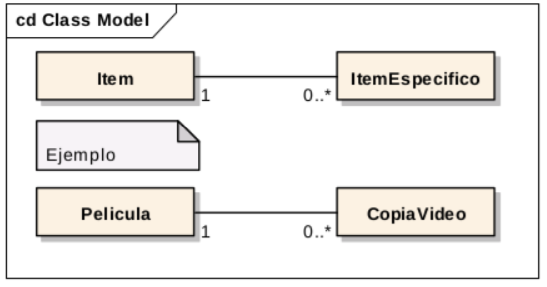
\includegraphics[width=0.6\textwidth]{img/PatronItemItemmEspecifico.PNG}
\end{figure}
\textit{Un titulo de una película puede ser un LineItem.}

\subsubsection*{Ensamble-Parte}
\begin{figure}[!htb]
    \centering
    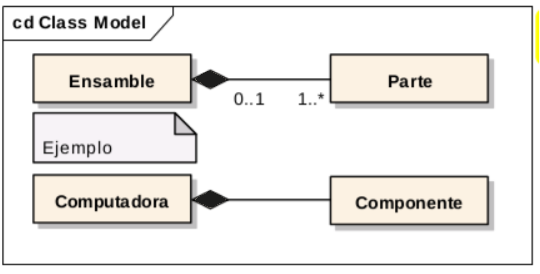
\includegraphics[width=0.6\textwidth]{img/PatronEnsambleParte.PNG}
\end{figure}

\subsubsection*{Contenedor-Contenido}
\begin{figure}[!htb]
    \centering
    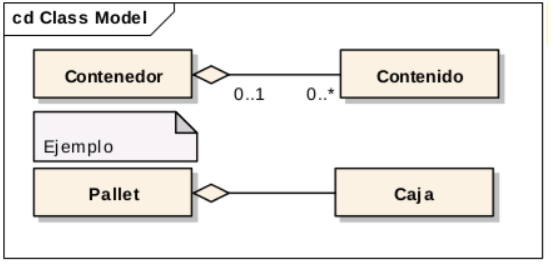
\includegraphics[width=0.6\textwidth]{img/PatronContenerdorContenido.PNG}
\end{figure}
\newpage
\subsubsection*{Grupo-Miembro}
\begin{figure}[!htb]
    \centering
    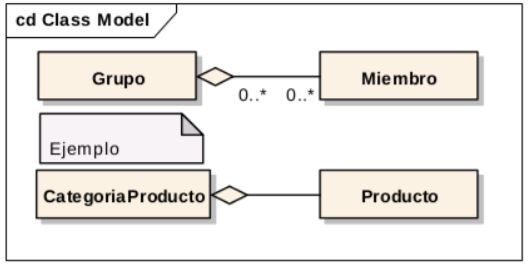
\includegraphics[width=0.6\textwidth]{img/PatronGrupoMiembro.PNG}
\end{figure}

\subsubsection*{Rol-Transacción}

\begin{figure}[!htb]
    \centering
    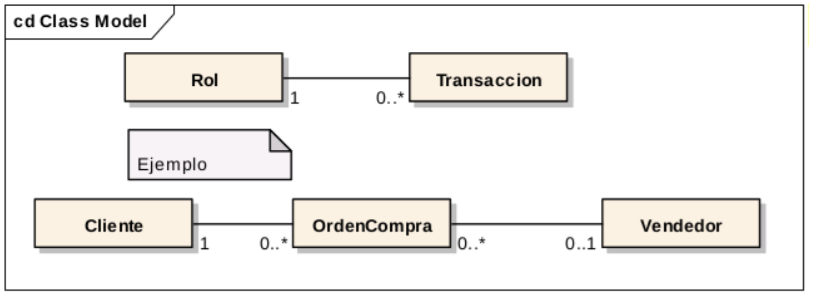
\includegraphics[width=0.6\textwidth]{img/PatronRolTransaccion.PNG}
\end{figure}
Le da la dinámica al negocio. \textit{Un orden de compra como registro de la compra}
\subsubsection*{Transacción-Lugar}

\begin{figure}[!htb]
    \centering
    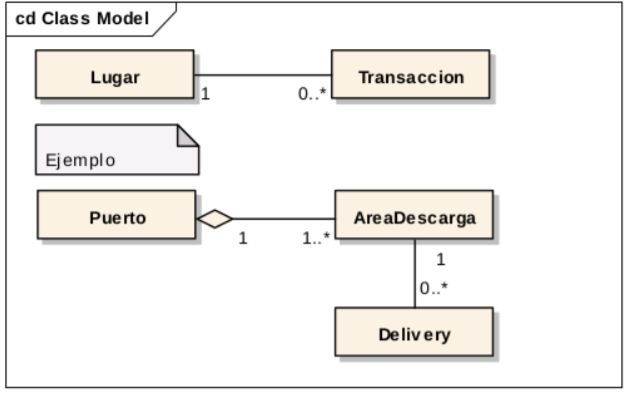
\includegraphics[width=0.6\textwidth]{img/PatronLugarTransaccion.PNG}
\end{figure}
Da dinámica del negocio también.
\newpage
\subsubsection*{Transacción-ItemEspecifico}

\begin{figure}[!htb]
    \centering
    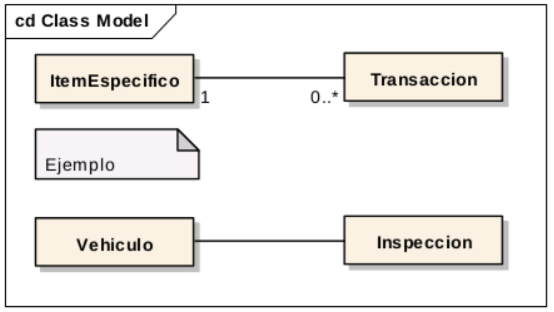
\includegraphics[width=0.6\textwidth]{img/PatronItemEspecificoTransaccion.PNG}
\end{figure}

\subsubsection*{ItemEspecifico-LineItem}
\begin{figure}[!htb]
    \centering
    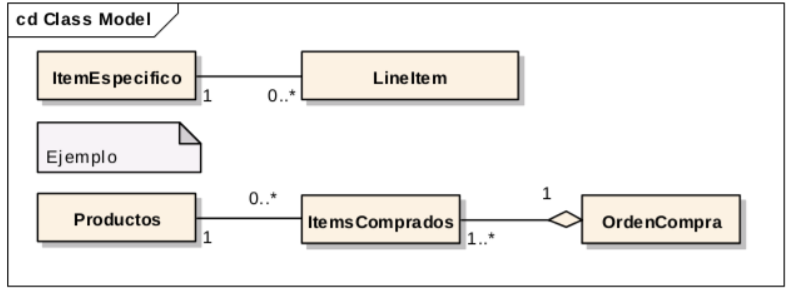
\includegraphics[width=0.6\textwidth]{img/PatronItemEspecificoLineItem.PNG}
\end{figure}

\subsubsection*{TransaccionCompuesta-LineItem}
\begin{figure}[!htb]
    \centering
    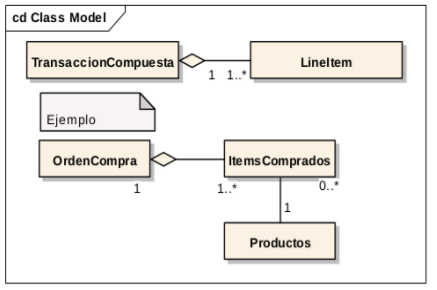
\includegraphics[width=0.6\textwidth]{img/PatronTransaccionCompuestaLineItem.PNG}
\end{figure}

\newpage
\subsubsection*{Transaccion-TansaccionCronologica}

\begin{figure}[!htb]
    \centering
    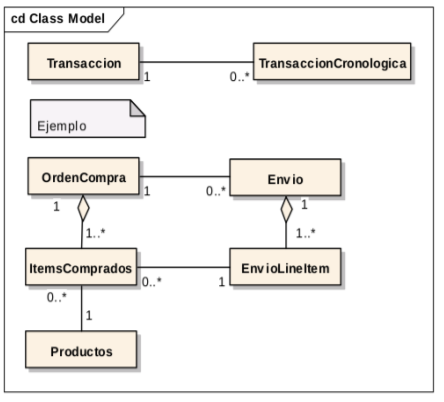
\includegraphics[width=0.6\textwidth]{img/PatronTransaccionTransaccionCronologica.PNG}
\end{figure}

\subsection*{Pasos para su búsqueda}
\begin{enumerate}
\item Preguntarse quiénes realizan tareas en este dominio/negocio, de esta forma se identifican actores y se les asigna un rol
\item Preguntarse qué tareas realizan, así se asignan transacciones
\item Preguntarse sobre qué objetos de negocio se realiza estas transacciones, así se asignan items específicos
\item Preguntarse qué transacciones deben realizarse antes que otras, así se asignan transacciones cronológicas
\item Preguntarse dónde se realizan las transacciones, así se asigna un lugar a estas transacciones
\item Preguntarse si los Items tienen identificación o no, para identificar si se usa Lines Items o no
\item No confundir transacciones de negocio con transacciones de sistema.
\end{enumerate}

La base que tiene que quedar en todo modelo de dominio es la siguiente.

\begin{figure}[!htb]
    \centering
    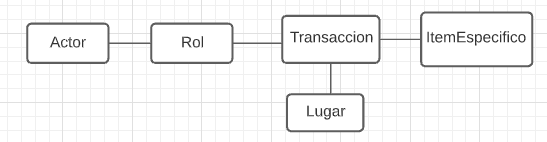
\includegraphics[width=0.8\textwidth]{img/BaseModeloDeDominio.PNG}
\end{figure}

\section{Reglas de negocio}

\begin{itemize}
\item Las reglas de negocio son las restricciones que gobiernan las acciones dentro de un dominio de negocio. En el modelo se traducen en reglas de colaboración. Estas se incorporan al modelo en restricciones a ser probadas en la colaboración entre los distintos objetos del modelo.
\item Si no se ubican en el modelo, el modelo esta incompleto.
\end{itemize}

Hay 5 tipos de reglas de negocio: 
\begin{itemize}
\item De tipo: \textit{Un medicamento puede ser cargado solo en un container refrigerado.}
\item De multiplicidad: \textit{Un pallet refrigerado puede contener hasta 10 cajas.}
\item De propiedad: Se refiere a validación o comparaciones. \textit{Un pago debe registrar un número válido de tarjeta de crédito, la temperatura de un container refrigerado debe ser menor a 0 grados centígrados.}
\item De estado: \textit{Una orden no debe ser entregada si antes fue cancelada.}
\item De conflicto: \textit{Un vuelo no puede ser programado en una puerta en un mismo horario que otro vuelo, un producto no puede ser sumado a una orden de compra de un menor de edad si la venta está prohibida a menores.}
\end{itemize}

\begin{figure}[!htb]
    \centering
    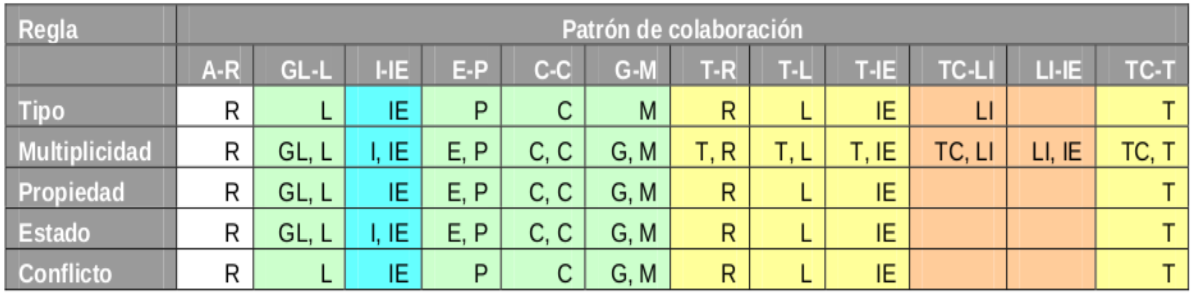
\includegraphics[width=0.8\textwidth]{img/ReglasDeNegocioSegunPatrones.PNG}
\end{figure}

\textit{Por ejemplo, la regla de tipo de Granlugar-lugar, la valida el lugar}. Si tiene ambos, involucra a ambos objetos.